\section*{Multiple Dimensions}

    Now that we've handled the 1-D case, we'll move into 2-D: now, we have \textbf{two} parameters, $\theta_1$ and $\theta_2$, as the input to $J$.
    
    \begin{figure}[H]
        \centering
            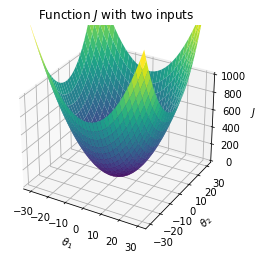
\includegraphics[width=70mm,scale=0.5]{images/gradient_descent_images/3dplot.png}
        
        \caption*{The "height"of your plot in 3D, is, again, your output! You want to move \textbf{downhill}.}
    \end{figure}
        
    \subsection*{Multivariable Local Approximation (Review)}
    
        Again, we rely on \textbf{calculus}. We want to move up to having more parameters: more \textbf{dimensions}. 
        
        Before, in 1-D, we found that, if you \textbf{zoomed} in enough on a function (using a "\textbf{local} view"), we could \textbf{approximate} it as a \textbf{straight line}, and move up or down that slope.
        
        There are \textbf{two} ways we can \textbf{approximate} like we want to in 2-D:
            \note{Remember that, by 2-D, we mean two \textbf{parameters}/inputs to $J$. If we add in the \textbf{height} of our function, that means our plot will \textbf{look} like 3-D!}
        
        \begin{itemize}
            \item First, we could turn it back into 1-D: we remove one variables.
            
            We do this by turning one variable constant: take $\theta_2=0$. Now, we have one free variable $\theta_1$. Same as 1-D.\\
        \end{itemize}
        
        \begin{concept}
            We can \gren{reduce} the number of \purp{variables} we have to work with, by holding some of them \gren{constant}. That way, we have a \purp{simpler} problem to work with.
            
            This is \purp{the same} as taking a single 2-D plane in a 3-D plot.
        \end{concept}
        
        \begin{figure}[H]
                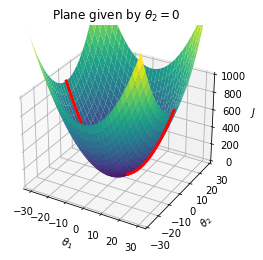
\includegraphics[width=70mm,scale=0.5]{images/gradient_descent_images/theta2_eq_0_unsliced.png}
                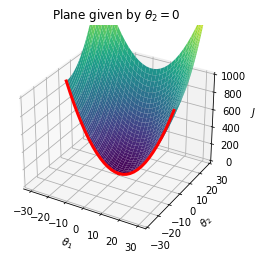
\includegraphics[width=70mm,scale=0.5]{images/gradient_descent_images/theta2_eq_0_sliced.png}
            
            \caption*{If we focus on a single plane of this surface, we end up with a \textbf{parabola}.}
        \end{figure}
        
        We can do the same the other way: we take $\theta_1=0$, and now we have a 1-D problem in $\theta_2$.
        
        \begin{figure}[H]
                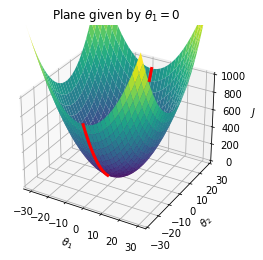
\includegraphics[width=70mm,scale=0.5]{images/gradient_descent_images/theta1_eq_0_unsliced.png}
                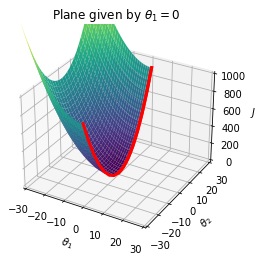
\includegraphics[width=70mm,scale=0.5]{images/gradient_descent_images/theta1_eq_0_sliced.png}
            
            \caption*{We can slice along the other axis as well!}
        \end{figure}

        Along each \textbf{axis}, $\theta_1$ and $\theta_2$, you can \textbf{approximate} our function as \textbf{two} different straight lines. Which leads into our next point...
        
        \begin{itemize}
            \item Second way: if we take the two perpendicular \textbf{lines} we got from each dimension, we can combine them into a \textbf{plane}.\\
        \end{itemize}
        
        \begin{concept}
            If we have \vocab{two input variables} (a 2-D problem), we can \purp{approximate} our surface as a \vocab{plane} if we \gren{zoom} in enough.
        \end{concept}
        
        These \textbf{approximations} will allow us to \textbf{optimize}.

    \subsection*{2-D: One dimension at a time}
        
        How do we \textbf{improve} our function $J$? Now that we have \textbf{two} dimensions, we have to store our change $\Delta \theta$ in a \textbf{vector}:
        
        \begin{equation}
            \Delta \theta
            =
            \begin{bmatrix}
                  \Delta \theta_1 \\ \Delta \theta_2 
            \end{bmatrix}
        \end{equation}
        
        This \textbf{complicates} things: we have two different things to consider \textbf{at once}.
        
        Well, the \textbf{simplest} way would be to treat it as a \textbf{1-D} problem, and do exactly what we did \textbf{before}. 
            \note{Note that we switched to \textbf{partial} derivatives, because we have \textbf{multiple} input variables $\theta_i$.}
        
        \begin{equation}
            \Delta \theta_1 = \pderiv{J}{\theta_1}
        \end{equation}
        
        Writing this in our \textbf{new} notation, we get:
        
        \begin{equation}
            \Delta \theta
            =
            - \eta 
            \begin{bmatrix}
                  \pderivslash{J}{\theta_1} \\ 0 
            \end{bmatrix}
        \end{equation}
        
        And then we would take a \textbf{step}, moving along the $\theta_1$ \textbf{axis}.
        
        \begin{figure}[H]
            \centering
                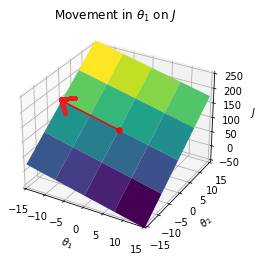
\includegraphics[width=70mm,scale=0.5]{images/gradient_descent_images/theta1_movement_plane.png}
            \caption*{We can move along $\theta_1$ just like on a line.}
        \end{figure}
        
        What if we treated this as a 1-D problem for the \textbf{other} variable, $\theta_2$?
        
        \begin{equation}
            \Delta \theta
            =
            - \eta 
            \begin{bmatrix}
                  0 \\ \pderivslash{J}{\theta_2} 
            \end{bmatrix}
        \end{equation}
        
        With this equation, we would be \textbf{moving} along the $\theta_2$ axis.
        
        \begin{figure}[H]
            \centering
                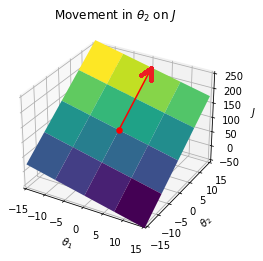
\includegraphics[width=70mm,scale=0.5]{images/gradient_descent_images/theta2_movement_plane.png}
            \caption*{We can do the same with $\theta_2$.}
        \end{figure}
        
        Why not move in \textbf{both} directions \textbf{at once}? We can \textbf{combine} our two derivatives: we'll add up our two steps.
        
        \textbf{Linearity} means that I can \textbf{add} them up without anything \textbf{weird} happening.
            \note{The relevant linearity rule: $L(x+y)=L(x)+L(y)$. In other words: taking two separate steps is the same as one big step.}
        
        \begin{equation}
            \Delta \theta
            =
            - \eta 
            \begin{bmatrix}
                  \pderivslash{J}{\theta_1} \\ 0 
            \end{bmatrix}
            - \eta 
            \begin{bmatrix}
                  0 \\ \pderivslash{J}{\theta_2} 
            \end{bmatrix}
        \end{equation}
        
        These can be combined because we're treating our function as a \textbf{flat} plane: if I move in the $\theta_1$ direction first, it doesn't change the $\theta_2$ slope, and vice versa.
        
        \begin{figure}[H]
        \centering
            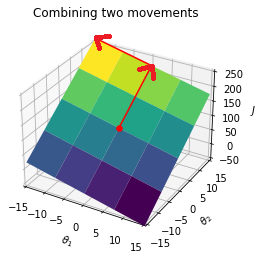
\includegraphics[width=70mm,scale=0.5]{images/gradient_descent_images/thetaboth_movement_plane.png}

            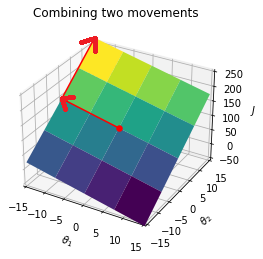
\includegraphics[width=70mm,scale=0.5]{images/gradient_descent_images/thetaboth_movement_plane_reversed.png}
                
            \caption*{Our plane being flat means we can take both operations, back-to-back! Notice that the order doesn't matter.}
        \end{figure}
        
        \begin{equation}
            \Delta \theta
            =
            - \eta 
            \begin{bmatrix}
                  \pderivslash{J}{\theta_1} \\ \pderivslash{J}{\theta_2} 
            \end{bmatrix}
        \end{equation}
        
        So, let's use that to optimize:\\
        
        \begin{kequation}
            In \vocab{2-D}, you can optimize your function $J$ using this rule:
            
            \begin{equation*}
                \red{ \theta_{new} } =  \blu{ \theta_{old} } 
                - \grn{ \eta } 
                \underbrace{
                    \begin{bmatrix}
                          \pderivslash{J}{ \blu{\theta_1} } \\ 
                          \pderivslash{J}{ \blu{\theta_2} } 
                    \end{bmatrix}
                }_{ \text{Using } \blu{ \theta_{old} } }
            \end{equation*}
            
            This is our \vocab{gradient descent} rule for 2-D.
        \end{kequation}
        
        This sort of approach makes some \textbf{sense}: if $\pderiv{J}{\theta_1}$ is \textbf{bigger} than $\pderiv{J}{\theta_2}$, that means that you can get \textbf{more benefit} from moving in the $\theta_1$ direction than $\theta_2$.
        
        So, in that case, your step will move more in the $\theta_1$ direction: it's a more \textbf{efficient} way to get a \textbf{better} hypothesis!
        
        But for now, we \textbf{don't know} that this is necessarily the \textbf{optimal} way to change $\theta$ - we'll explore that later.